\documentclass[12pt,a4paper]{article}
\usepackage{enumerate}
\usepackage{fullpage}
\usepackage{amsmath}
\usepackage{graphicx}
\usepackage{verbatim}
\usepackage{parskip}

% Stuff for dot2tex
\usepackage[x11names, rgb]{xcolor}
\usepackage[utf8]{inputenc}
\usepackage{tikz}
\usetikzlibrary{snakes,arrows,shapes}


\title{Stats 391 Project}
\author{By \\ Henry Baba-Weiss, Bill Cauchois, Coral Peterson, and Michael Sloan}
\date{\today}

\begin{document}

\maketitle
\pagebreak

\section { Background }

Tweets are very short messages posted to the online micro-blogging service Twitter. By convention less than 140 characters in length, tweets may also contain Twitter-specific idioms such as hashtags and @ mentions.  The brevity and concision of Twitter make it a potentially interesting source of information for applying more naive statistical methods and learning techniques.  Many of the Tweets are written to be consumed without additional context, making them ideal targets for more simplistic statistical methods.

\section { Description }

The goal of our project is to apply statistical tools to build a model which predicts the ``sentiment'' of tweets.  This sentiment is dichotomized into just two categories: ``positive'' and ``negative''.  The positive category is used for posts that would otherwise go into a neutral category, if it existed. By mapping each word in the tweet to the amount that the term seems to be biased towards positive or negative tweets, %% TODO


\section { Maths }

\subsection { Naive Bayes }

The ``Naive Bayes classifier'' takes the following form:

\begin{align*}
p(C \vert F_1,\dots,F_n) = \frac{1}{Z}  p(C) \prod_{i=1}^n p(F_i \vert C)
\end{align*}

This formula comes from assuming that the conditions, $ F_n $, are independent.  The $ Z $ is a scaling factor, which is irrelevant for the purposes of comparison.  This allows us to extract the compound probability, $ p(F_1,\cdots,F_n) = \prod_{i=1}^n p(F_i) $ from the usual formula for Bayes' theorem:

\begin{align*}
p(C \vert F_1,\dots,F_n) & = \frac{p(C) p(F_1,\dots,F_n\vert C)}{p(F_1,\dots,F_n)}    \\
                         & \approx \frac{p(C) \prod_{i=1}^n p(F_i \vert C)}{p(F_1,\dots,F_n)} \\
                         & \approx \frac{p(C) \prod_{i=1}^n p(F_i \vert C)}{Z}
\end{align*}
(Where $ Z = p(F_1,\cdots,F_n) $ )

In essence, this means that the likelihood of a given outcome is the product of the probabilities contributed by each of the predictors.  $ Z $ can be disregarded, because usually we are interested in comparing two outcomes.  For our usage here, we will assume that $ C_1 $ and $ C_2 $ are disjoint, which is given by our problem statement dichotomizing ``Positive'' and ``Negative'' sentiment.  In order to figure out which is more likely given all of $F_n$, we could calculate:

\begin{align*}
  & \frac{ p(C_1 \vert F_1,\dots,F_n) } { P(C_1 \vert F_1,\dots,F_n) + P(C_2 \vert F_1,\dots,F_n) } \\
  & \\
  \approx & \frac{\frac{p(C_1) \prod_{i=1}^n p(F_i \vert C_1)}{Z}}{\frac{p(C_1) \prod_{i=1}^n p(F_i \vert C_1)}{Z} + \frac{p(C_2) \prod_{i=1}^n p(F_i \vert C_2)}{Z}} \\
  & \\
  \approx & \frac{p(C_1) \prod_{i=1}^n p(F_i \vert C_1)}{p(C_1) \prod_{i=1}^n p(F_i \vert C_1) + p(C_2) \prod_{i=1}^n p(F_i \vert C_2)}
\end{align*}

This results in a distribution on a discrete binary variable (the denominator specifies the domain that we're concerned with - we must be inhabiting either $ C_1 $ or $ C_2 $).  The assumption that $ C_1 $ and $ C_2 $ are disjoint allows us to express the overall probability of inhabiting the 

$ p(C_1) $ is referred to as the ``prior'', or the probability of $ C_1 $, regardless of other information.  This is an interesting aspect of the Naive Bayes classifier - achieving better results by ``starting'' with an appropriately biased assumption.

Our actual implementation does not use this form of the equation, as we're more interested in the comparison between $ P(C_1 \vert F_1,\dots,F_n) $, rather than their absolute values.  As such, we can take a log of both sides, while maintaining ordering (of positive values, which probabilities are):

\begin{align*}
p(C_1 \vert F_1,\dots,F_n) & \stackrel{\text{?}}{\leq} p(C_2 \vert F_1,\dots,F_n) \\
log p(C_1 \vert F_1,\dots,F_n) & \stackrel{\text{?}}{\leq} log p(C_2 \vert F_1,\dots,F_n) \\
log p(C_1) \prod_{i=1}^n p(F_i \vert C_1) & \stackrel{\text{?}}{\leq} log p(C_2) \prod_{i=1}^n p(F_i \vert C_2) \\
log p(C_1) + \sum_{i=1}^n log p(F_i \vert C_1) & \stackrel{\text{?}}{\leq} log p(C_2) + \sum_{i=1}^n log p(F_i \vert C_2) \\
\end{align*}

\subsection { Sparsity assumptions }

A more recent development in sensor post-processing / learning models is an idea that's referred to as ``compressive sensing'', which attempts to recover more accurate models by assuming that the process being studied is ``sparse''.  Many continuous optimization problems can be posed in terms of something similar to the $ L_2 $ norm.  This norm creates surfaces that resemble a parabola - the slope near zero is low.  The key observation of ``compressive sensing'' is that optimizing things that much more resemble the structure of the linear norm, $ L_1 $, creates more extreme slopes at the origin.  This encourages values to be set to zero, hence the word ``sparsity''.  Correspondingly, this encourages the non-zero elements to be more significant than they would be otherwise.

The reason these concepts are relevant to our study is that it gives a framework within which to address the issue that many of the $ p(F_i \vert C) $ probabilities are close to $ 0.5 $ or are supported by few samples.


\subsection{ Graphical Models }

The study of graphical models involves the crossover between graph theory and probability theory, and gives a uniform perspective of many techniques for creating models and categorizers.  These models express dependencies between states of various nature relating to a system - in the case of ``Partially Observable Markov Decision Processes'', this includes observations and states.  The dependencies among the states indicate the temporal interdependencies of the states, while also being informed by the observations.  The current state of the belief distribution is used as an input, along with these observations, to evaluate the joint probabilities at each state, of now inhabiting that state.  Thankfully, our model does not need to worry about anything quite like these temporal dependencies (but if we worried about context, something like this would be needed!).

Anyway, since our system is merely Naive Bayes, it can be expressed quite trivially as a graphical model:

\input { figs/fig1.tex }

\section{ Implementation }

The implementation of our project can be broadly divided into several different components. Before performing any classification, we first had to collect data and then label that data. We implemented a \textbf{scraper} in Python to aggregate raw tweets from Twitter's feed of recent tweets. Next, we used several different methods to label the tweets as positive or negative in order to create a training set for our classifier. These methods included \textbf{Mechanical Turk}, a web-based service that lets you pay others to perform classification; \textbf{manual console categorization}, wherein we manually classified tweets using a console program; and \textbf{manual web-based categorization}, wherein we manually classified tweets using a web application. Now that we had labeled data, the next challenge was \textbf{lexing} that data to create a bag of words representation for each tweet. Finally, we built our \textbf{Bayesian categorizer}.

\subsection { Scraper }

The first component we built was a scraper to grab random tweets from Twitter. To do so, we used the \texttt{twitter.Api().GetPublicTimeline()} method on the Twitter Python API, which in turn uses HTTP REST to grab the most recent tweets from the public, global timeline. One problem we ran into was that not all of these tweets were in English. In order to discard tweets that weren't in English, we relied upon a Java library called TextCat that performs text categorization into different languages. So we created a small program that read in a tweet, and outputted the language in which that tweet was written. Then, we could call into this program from Python and use it to discard any tweet for which the output from TextCat was \emph{not} ``english''. The output from our scraper was stored in comma-separated values format. Here is an example listing (including the header):

\begin{verbatim}
name,text
Marcus Graham ,Go somewhere then RT @NurseJessica_88: Im seriously needing to get out the house
Brett taborelli,Here it goes.
Jessica Stein,Thank god I'll be waking up in sea isle instead of havertown tomorrow
\end{verbatim}

\subsection { Mechanical Turk }

Our first approach to solving the problem of labeling our tweets relied upon a service called Mechanical Turk. Mechanical Turk bills itself as ``an online crowdsourcing marketplace''. Crowdsourcing is a recently coined term that refers to outsourcing tasks to a distributed group of people, usually via the internet. Basically, MTurk enables users known as Requesters to post tasks known as HITs (human intelligence tasks) for a distributed force of Workers to perform for a small fee. There are several different types of HITs, but the type we were interested in was the classification HIT, wherein a Worker assigns one of $n$ categories to a piece of data. MTurk turned out to be relatively easy to use. A web interface allows you to upload a dataset in comma-separated values format and turn it into a series of HITs, which you can then deploy to the marketplace. You must pre-pay by depositing money into an MTurk account, and then your HITs are live. The only problem we faced with this approach was the cost: it cost about $\$1.00$ to classify 40 tweets. For us, this was prohibitively expensive, and thus we developed some manual classification methods for ourselves.

\subsection { Manual Console Categorization }

The console manual categorization program is written in Python, and allows us to respond negative or positive for a constant stream of posts stored by the scraper.  When the program starts, it looks like this, providing instructions and an initial tweet to categorize:

\begin{verbatim}
enter n for negative, p for positive
vvvvvvvvvvvvvvvvvvvvvvvvvvvvvvvvvvvvvvvvvvvvvvvvvvvvvvvvvvvv
Reality is an illusion that occurs due to lack of alcohol
\end{verbatim}

This is a real tweet encountered while using the tool -- one thing we learned from this project is that Twitter users are hilarious and sometime sad.  We were very surprised by the quantity of posts that fell squarely within the negative category.  Here's a portion of a contiguous session with the tool:

\begin{verbatim}
____________________________________________________________
vvvvvvvvvvvvvvvvvvvvvvvvvvvvvvvvvvvvvvvvvvvvvvvvvvvvvvvvvvvv
Waiting For The Sun To Go Awayy  So I Could Go Run!
classified as NEGATIVE
____________________________________________________________
vvvvvvvvvvvvvvvvvvvvvvvvvvvvvvvvvvvvvvvvvvvvvvvvvvvvvvvvvvvv
I always see people get mad and into argument over the littlest things  and
  I hate arguing .
classified as NEGATIVE
____________________________________________________________
vvvvvvvvvvvvvvvvvvvvvvvvvvvvvvvvvvvvvvvvvvvvvvvvvvvvvvvvvvvv
Finally I have convinced her to abandon her husband  and make our lives one.
classified as NEGATIVE
____________________________________________________________
vvvvvvvvvvvvvvvvvvvvvvvvvvvvvvvvvvvvvvvvvvvvvvvvvvvvvvvvvvvv
he was not sitting on a boar
classified as POSITIVE
____________________________________________________________
vvvvvvvvvvvvvvvvvvvvvvvvvvvvvvvvvvvvvvvvvvvvvvvvvvvvvvvvvvvv
Stressing over history #TheUsual
classified as NEGATIVE
____________________________________________________________
vvvvvvvvvvvvvvvvvvvvvvvvvvvvvvvvvvvvvvvvvvvvvvvvvvvvvvvvvvvv
So James is a whore now? Smh
classified as NEGATIVE
____________________________________________________________
vvvvvvvvvvvvvvvvvvvvvvvvvvvvvvvvvvvvvvvvvvvvvvvvvvvvvvvvvvvv
The most interesting birthday yet... thanks to a very beautiful friend of mine...
  *all smiles*
classified as POSITIVE
\end{verbatim}

Some were also far more ridiculously negative than the examples here.  For more neutral posts, or random posts that likely require more context, the categorization positive was used, as can be seen by the positive categorization given to ``he was not sitting on a boar''.

\subsection { Manual Web-Based Categorization }

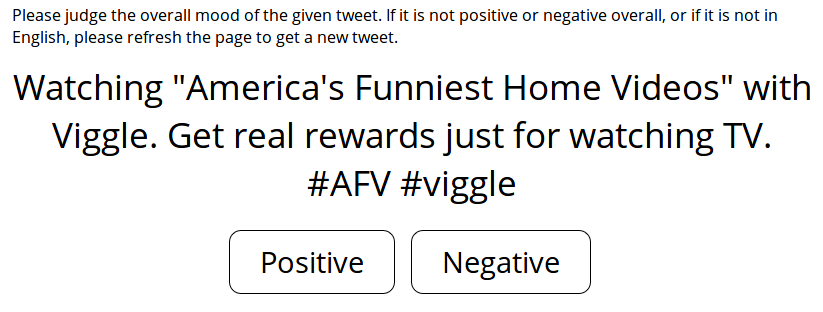
\includegraphics[width=470px]{figs/web_cat.png}

\subsection { Lexer }

One of the main assumptions of this project is that the chosen lexical units, in this case, words, are independent predictors of the classification of the Tweet.  This assumption cannot be correct, for something as complicated as language, but this does imply that the choice of partitioning the lexical units does matter.  Even after we have decided to use single-word lexemes, this leaves us with a few choices:

\begin{enumerate}[1)]
\item Do we maintain capitalization?
\item How do we handle ``\#hash'' keywords?
\item How do we handle emoticons like ``:)'', ``:('', and ``:')'' - these are the closest thing to a direct encoding of sentiment - so preserving them for the analysis is important!
\item How do we handle ``\&gt;'', ``\&lt;'', and other HTML entities?  These particular examples are interesting, because they are conventionally used to indicate something good (``\&gt;'') or bad (``\&lt;'').
\item How is regular punctuation reported?
\end{enumerate}

Our solution to these considerations was to break the text on the whitespace / punctuation characters, and lowercase everything.  In order to reasonably handle HTML entities, ``\&'' would be included with any tokens it prefixes, while ``;'' is ignored.  The other punctuation is grouped with adjacent punctuation, and each group reported as a separate word.  This handles the extremely informative punctuation such as emoticons, while also handling regular punctuation.  For example, it can be imagined that ``!'' might oftentimes terminate positive tweets, while ``...'' is used to terminate negative tweets.

\subsection { Bayesian Categorizer }

\subsection { Max-Uncertainty Queue }

One issue with this project is that, similarly to many studies, there is cost associated with taking additional samples.

In the case Mechanical turk, the cost was $ \$1.16 / 40 \text{ tweets} ~ \$0.029 \text{ tweets}^{-1}$. 

%TODO: consider measuring this better.

In the case of using the manual categorizer, we found that we could categorize tweets at about a rate of about $ 15 \text{ tweets} / \text{min} $.  This means that with a solid hour of work, we could categorize 900 tweets.  In order to compute what this means for our price per tweet, we first need an estimate of the value of our time.  If our time is worth the pay of a typical entry-level fulltime software engineer, $ \$40 / \text{hr} $, then each tweet costs $ \$40 \text{min}^{-1} / ( 900 \text{ tweets} * \text{min}^-1 \approx \$0.045 * \text{tweets}^-1 $.  However, we are all in school!  Perhaps it would be more appropriate to use the amount made as a TA: $ \$10.50 * \text{min}^{-1} / ( 900 * \text{tweets} * \text{min}^{-1} ) \approx \$0.015 $.  This is around half as much as the cost of Mechanical Turk, which incentivized us to do more manual than ``mechanized'' sampling.

Either way, it would be cool to make the most of the resource expenditure involved in categorization.  An interesting way of approaching this problem would be to write it down as an optimization problem that relates the cost of data collection with the potential for information gain:

\section { Results }

In the end, we collected 627 data points, including 354 positive categorizations and 272 negative categorizations. This breakdown is illustrated in the following graph:

\begin{center}
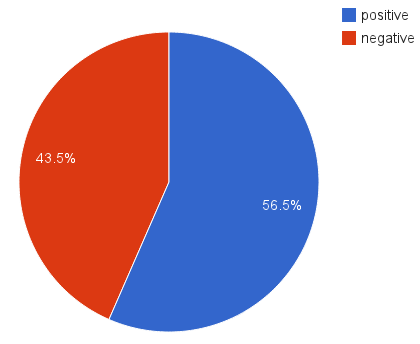
\includegraphics[width=300px]{figs/pos_neg_breakdown.png}
\end{center}

Our classification accuracy is summarized by the following table:

\begin{tabular}{|l|l|}
\hline
\emph{Dataset} & \emph{Accuracy} \\ \hline
Training & 98.2\% \\ \hline
Test & 69.84\% \\ \hline
\end{tabular}

A more detailed breakdown is as follows:

%TODO: tables, charts, and graphs.

\subsection { Speculation }

%TODO: figure out where to put this / rename.

Tweets use ``hash-tag'' prefixes of words or compounded words in order to indicate some key-word relevant to the contents of your tweet.  In other words, this is a way to even further reduce the amount of content potentially included in your posts, while connecting your post to others'.


\section { Future Work}

Some ideas for enhancements:

\begin{enumerate}[1)]
\item Use bi-grams / tri-grams.  Instead of just making a distinct choice here, to use, say, bi-grams instead of uni-grams as the unit of association, it would be interesting to try to mix the categories.  When a particularly 

\item Use more sophisticated models to infer distributions that observe a co-dependency on terms.  In other words, find cases in which the presence of two words in the same tweet is significant, whereas each in isolation is not.

\item Use more sophisticated ways of extracting structure from the individual tweets.  Instead of parsing into tokens that are considered independently, parse into a tree that gives the actual relational structure of the text.  This could then be used to run some sort of trained semantic interpretation of the content.  One way in which this could dramatically affect results is by noticing negations like ``not'', which can entirely invert the sentiment of a Tweet.

\item Use context derivable from the edges derivable from the hash-tag / conversational graph.  This would further inform the previous enhancement idea.
\end{enumerate}

In essence, these further enhancements are each a more sophisticated usage / implementation of NLP (natural language processing) techniques, that would generically enhance many related categorization tasks.

\end{document}
